\section{Appendix}
\label{sec:appx}
\subsection{Cost estimates}

The cost estimates for drilling pipes downstream of the Hall A beam dump are based on a budgetary bid for a single 16" pipe at location C indicated in 
Fig.\,\ref{fig:ds-area}. A cross section of the pipe (or ``well") is shown in Fig.\,\ref{fig:Well_Section_Bid}. 
The budgetary quote was adjusted by Suresh Chandra (JLab Facilities) to account for additional effort/work needed to complete the 
project. The resulting cost estimate is shown in Fig.\,\ref{fig:Preliminary_Cost_Estimate_16_Inch_pipe-Rev1}. The following
items were included in the cost:
\begin{itemize}
\item concrete slab on grade as a base for experimental test
\item ground exploration in advance of drilling
\item air blower to keep the well dry during test
\item drilling of the hole proper; installing a pipe suitable for use as a guide for the detector apparatus
\item backfill and compaction
\item generator (on loan from facilities) to provide temporary power for one-week test (3KVA).
\end{itemize}

Based on the budgetary bid, two cost estimates were made for 10" pipes based on previous experience with such similar projects. The estimates are shown in 
Figs.\ref{fig:Preliminary_Cost_Estimate_10_Inch_pipe} and \ref{fig:Preliminary_Cost_Estimate_for_two_10_Inch_pipes} at locations B and C of  Fig.\,\ref{fig:ds-area}.
Given that the muon rate changes considerably with
distance to the dump, we believe that two pipes are necessary to reliably understand the rate measurements. The estimated cost to drill two 10" pipes is \$40k. 
The typical time schedule for completing the project would be 8 weeks to prepare the contract, 6 weeks to award, and 6 weeks to complete the work, i.e. five months
total.

\begin{figure}[thp] 
\center
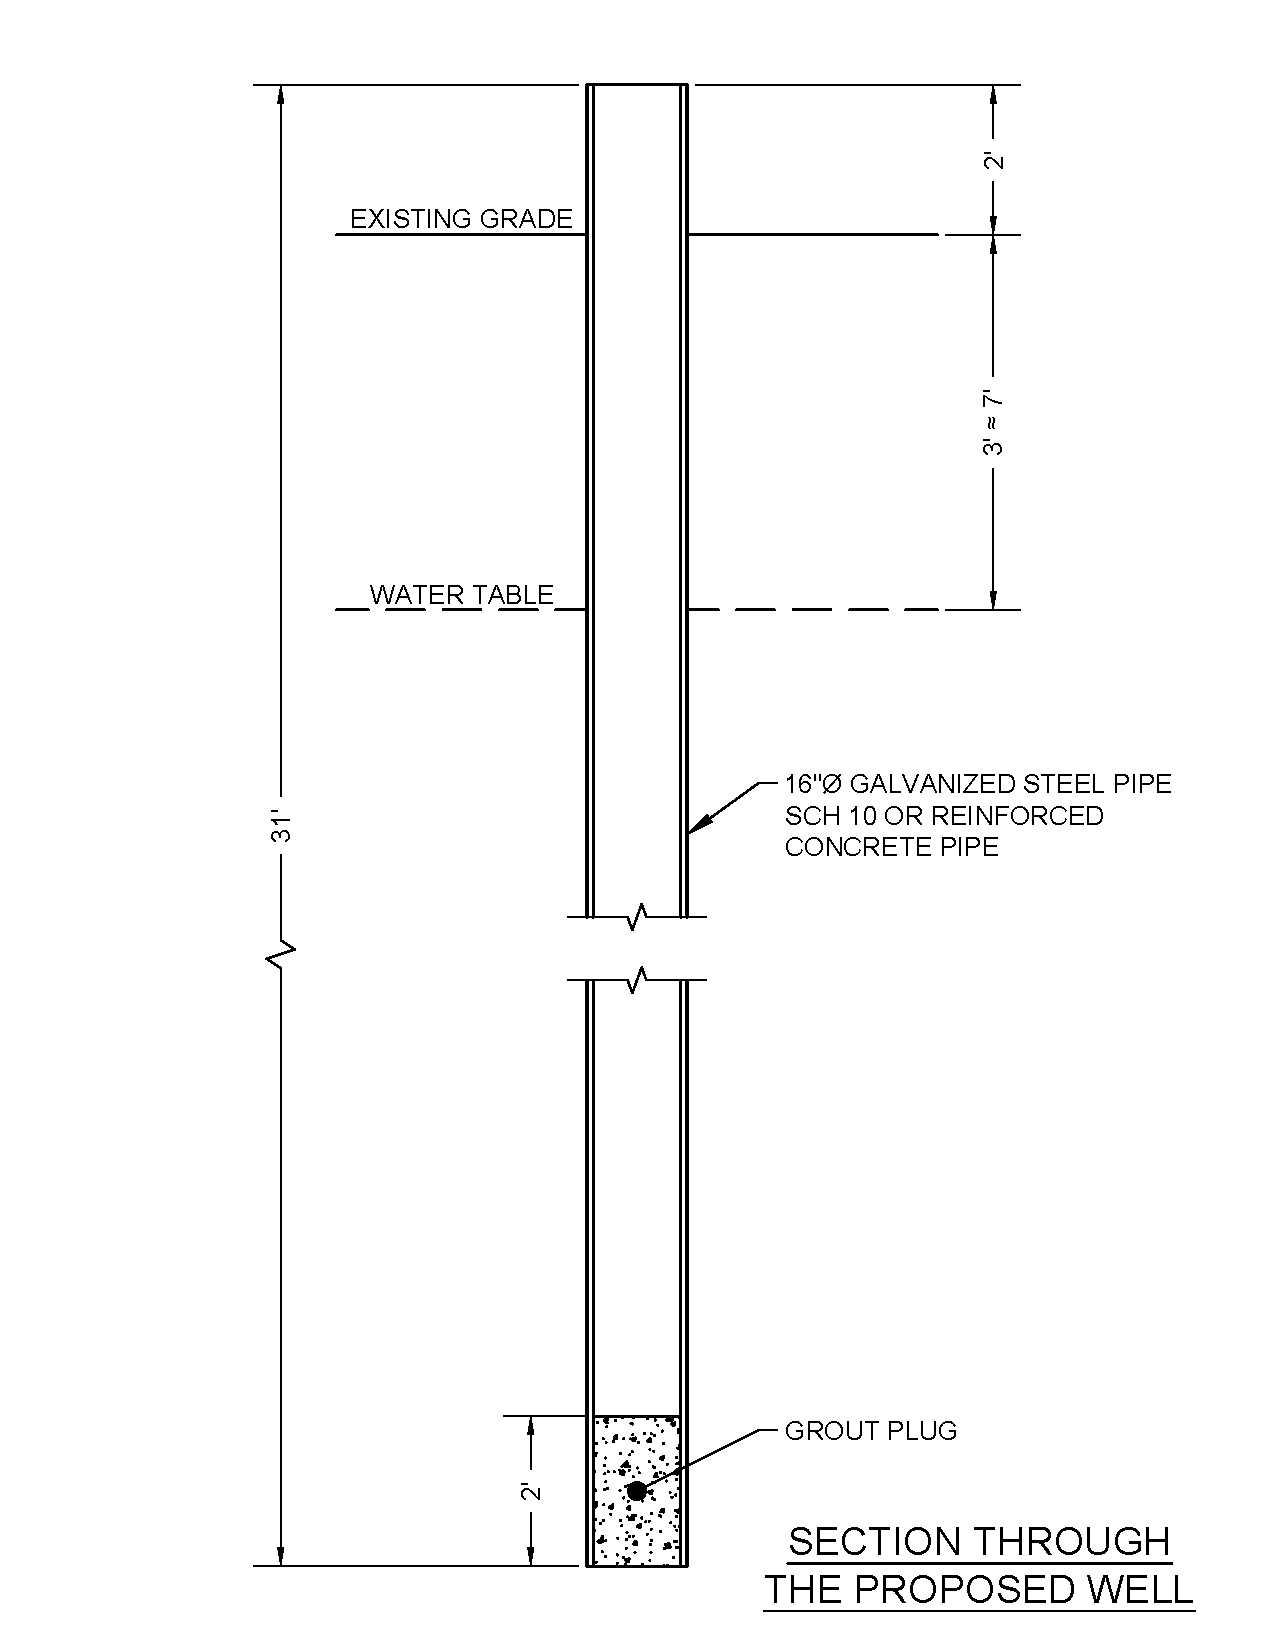
\includegraphics[width=8cm,clip=true]{figs/Well_Section_Bid.pdf}
\caption{Preliminary cost estimate for a single 16" pipe.}
\label{fig:Well_Section_Bid}
\end{figure}

\begin{figure}[thp] 
\center
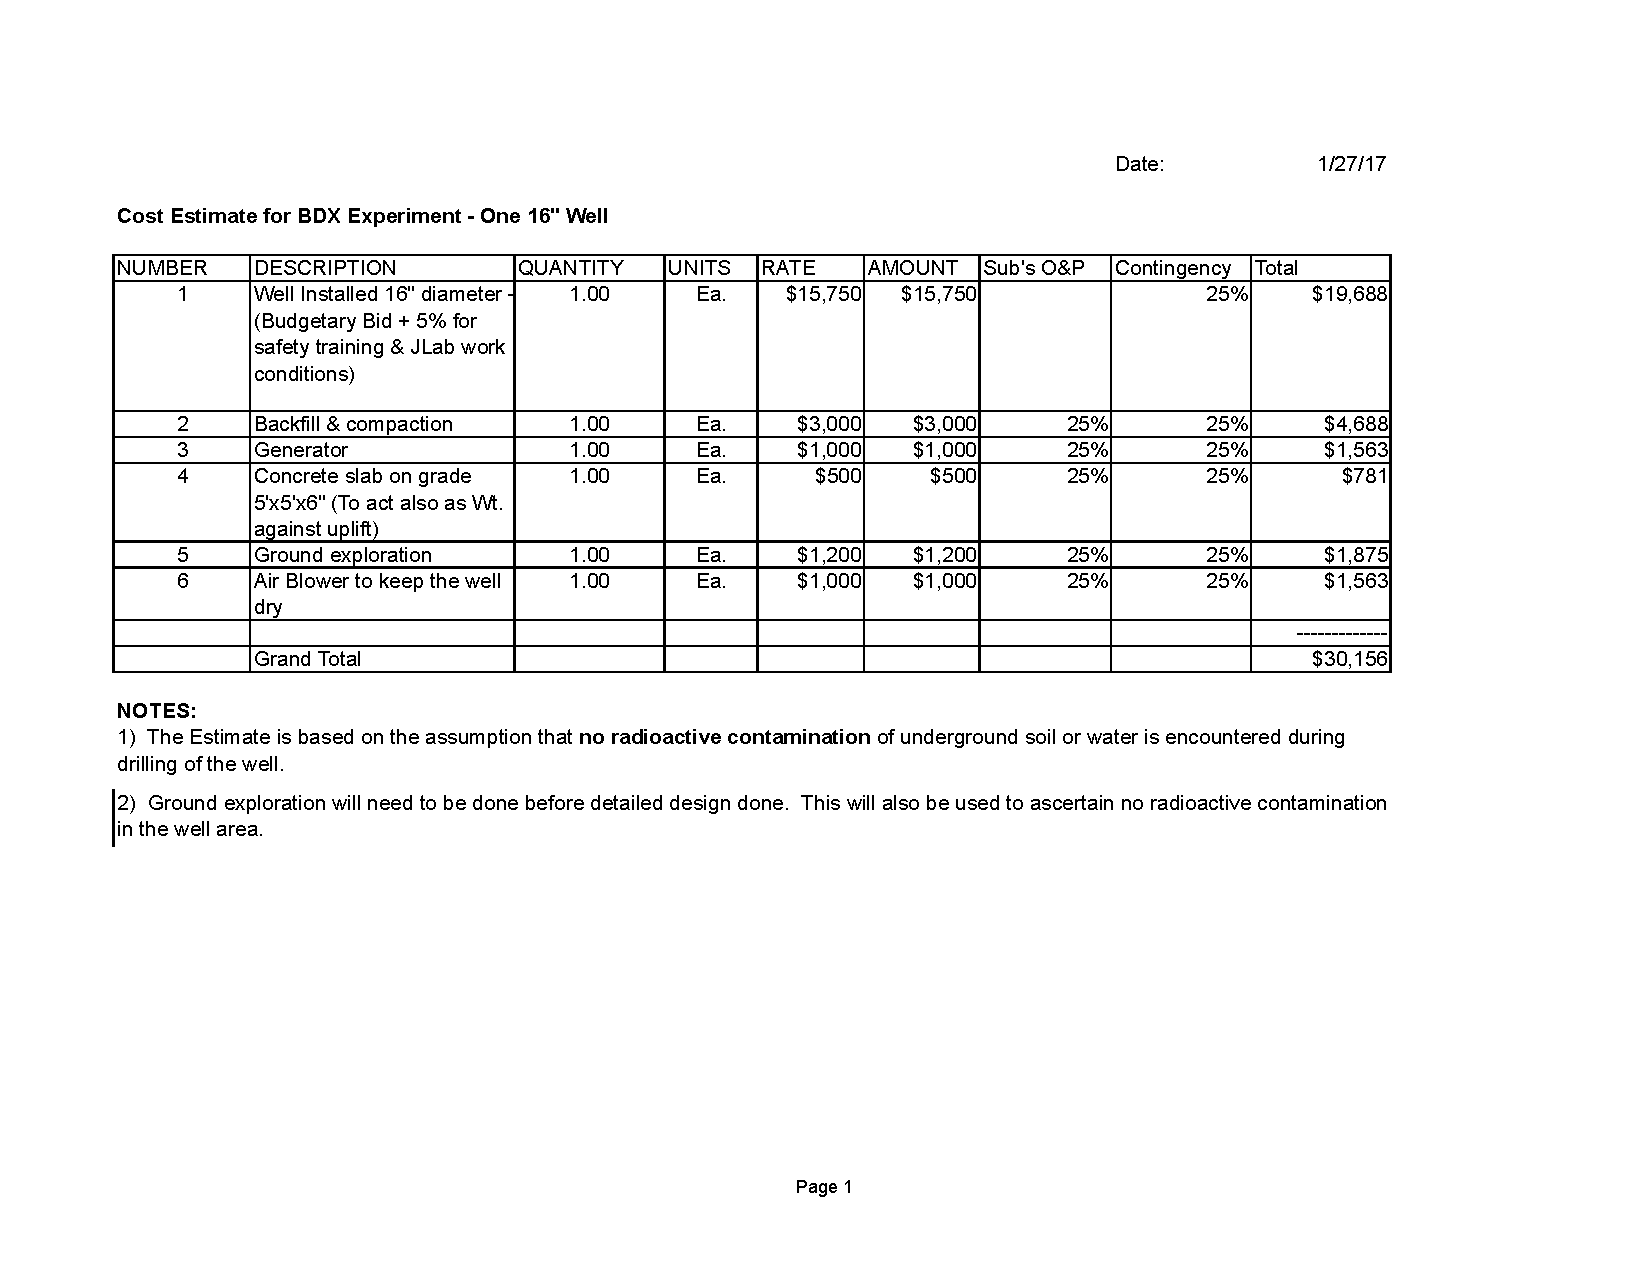
\includegraphics[width=17cm,clip=true]{figs/Preliminary_Cost_Estimate_16_Inch_pipe-Rev1.pdf}
\caption{Preliminary cost estimate for a single 16" pipe.}
\label{fig:Preliminary_Cost_Estimate_16_Inch_pipe-Rev1}
\end{figure}

\begin{figure}[thp] 
\center
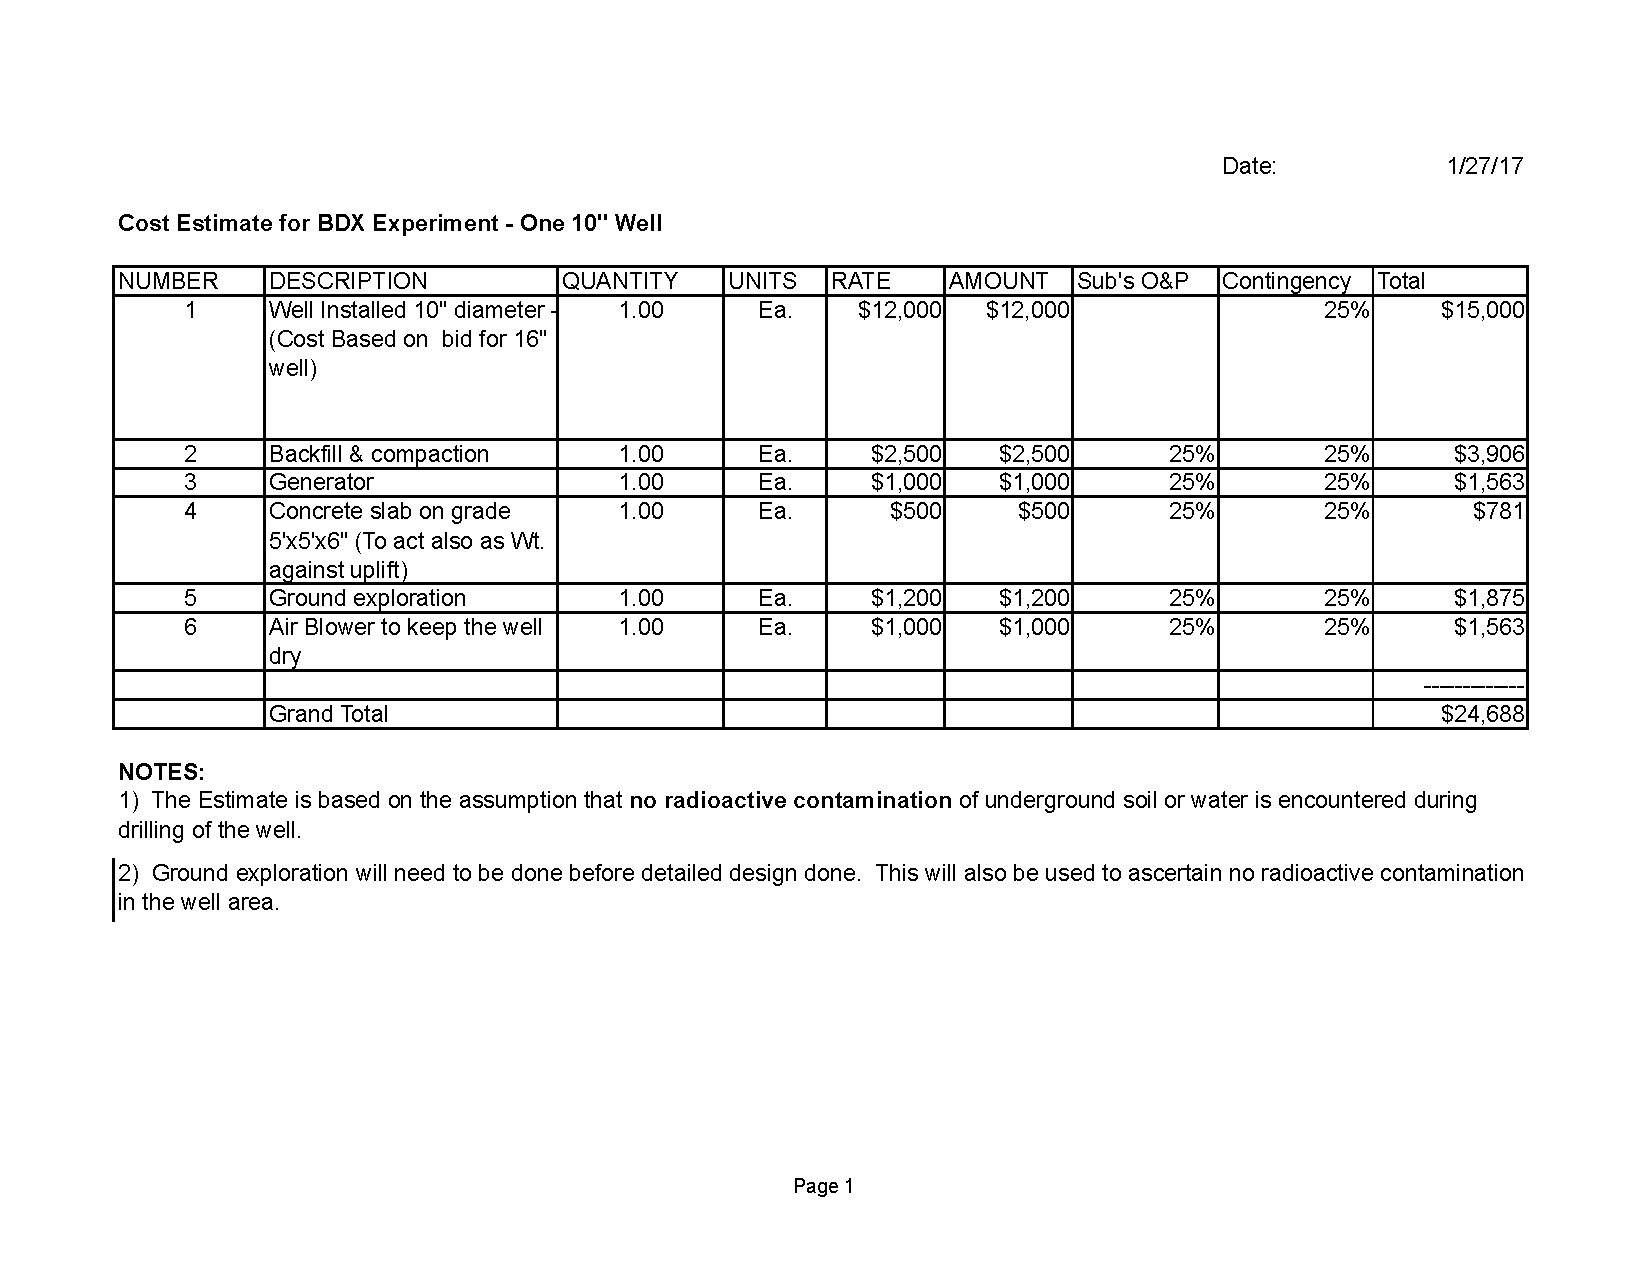
\includegraphics[width=17cm,clip=true]{figs/Preliminary_Cost_Estimate_10_Inch_pipe.pdf}
\caption{Preliminary cost estimate for a single 10" pipe.}
\label{fig:Preliminary_Cost_Estimate_10_Inch_pipe}
\end{figure}

\begin{figure}[thp] 
\center
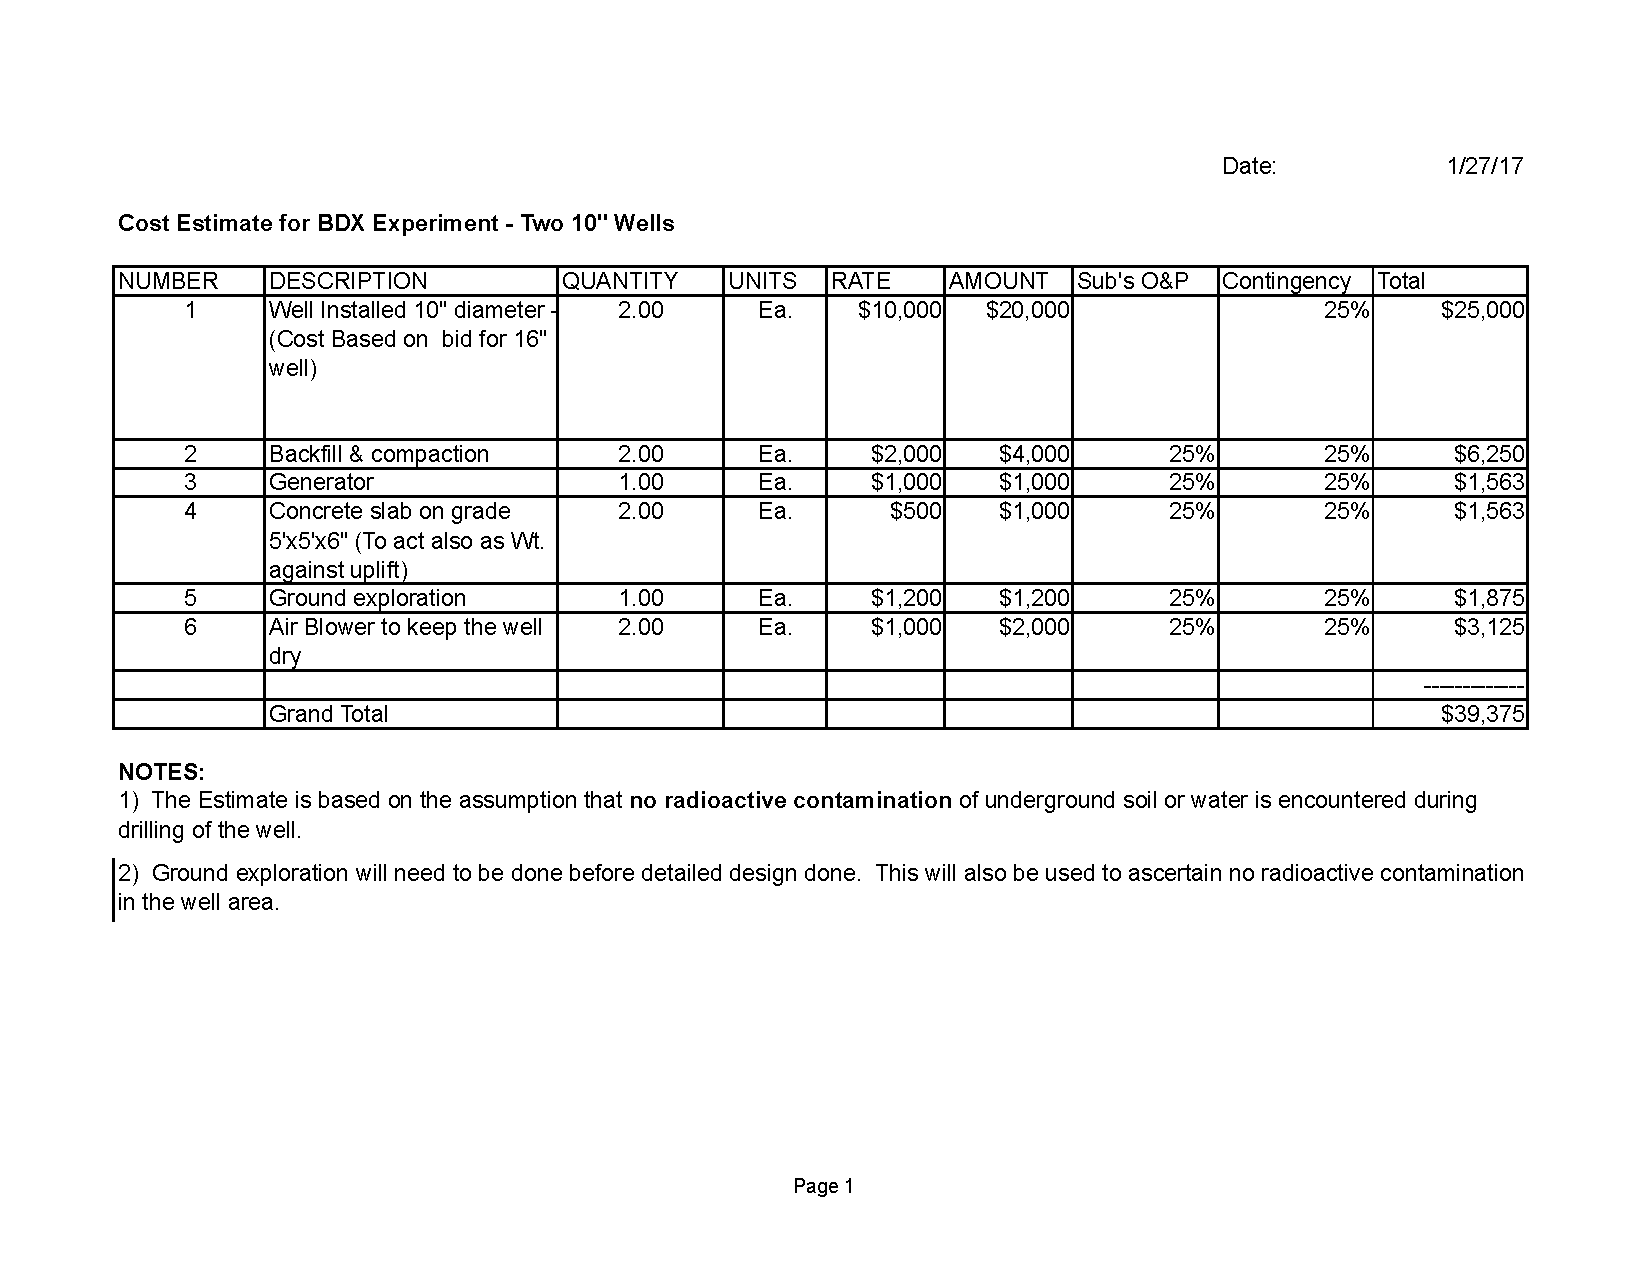
\includegraphics[width=17cm,clip=true]{figs/Preliminary_Cost_Estimate_for_two_10_Inch_pipes.pdf}
\caption{Preliminary cost estimate for two 10" pipes.}
\label{fig:Preliminary_Cost_Estimate_for_two_10_Inch_pipes}
\end{figure}


\subsection{Work- \& time-plan}
The two wells  will be drilled in locations {\bf B} and {\bf C} in the area downstream of the Hall-A beam-dump as shown in Fig~\ref{fig:ds-area} by inserting a 10" pipe as described in the previous Section. The test would  
run during the day, approximately for 4 calendar days \footnote{Assuming 8h day shifts only and  50$\%$ efficiency of CEBAF, this corresponds to less than 1 PAC days.}.
The test would be conducted during a time that 11-GeV beam with relatively steady current (between 1 and 100$\mu$A) is delivered  to Hall A.
The detector will be lowered in the pipe and positioned at different depths measuring counting rates at each setting. Table~\ref{tab:test} shows the expected CsI(Tl) rates and collected statistics.\
The beam-on status and the beam current are the only 
relevant accelerator information,  accessible off-line by  EPICS values stored in the  database\footnote{Synchronisation between BDX-Hodo DAQ and EPICS data  is required  at level of 1s.}. About 10 minutes of stable beam ($\frac{\Delta I_{Beam}}{I_{Beam}}<10\%)$ will  be enough to asses the relationship between beam current and detected muon rate and establish a normalization factor. 
If possible  we would like to take data at more than one beam current to check that the count rates scale.
This  would require 1h of dedicated beam-time  coordinated with the Hall-A physics program to change the beam current by a factor of 10.
Since the pipes will remain in place, it is worth noting that it will be possible to plan other opportunistic measurements with different Hall-A beam current/energy  set-ups.
 \begin{table}[htp]
\caption{Proposed test configuration}
\begin{center}
\begin{tabular}{|c|c|c|c|c|}
\hline\hline
\multicolumn{5}{r}{Preparation, quick scan at different depth,   $\sim$ 3h } \\
\hline
Position  &Depth  (cm)& Rate$_{Crystal} (kHz)$  &Run time (mn) & N$_{Evnt}$ collected (M)  \\
\hline\hline
 {\bf B} & 0 &  20 & 10 & 6\\
 \hline
 {\bf B}  & 40 &  10 & 20 & 6 \\
 \hline
 {\bf B}  & 80 &  4 & 40 & 5\\
 \hline
\multicolumn{5}{|r|}{Total time    $\sim$ 2h }\\
 \hline\hline
\multicolumn{5}{r}{Configuration change  $\sim$ 3h } \\
 \hline\hline
 {\bf C} & 0 &  2.8 & 30 & 5\\
 \hline
 {\bf C}  & 40 &  1.4 & 60 & 5 \\
 \hline
 {\bf C}  & 80 &  0.6 & 120 &4.5\\
 \hline
\multicolumn{5}{|r|}{Total time    $\sim$ 4h }\\
 \hline\hline
\end{tabular}
\end{center}
\label{tab:test}
\end{table}

